\begin{frame}{Part 2 Activity: A teammate hands you a folder}
  \vfill
  \begin{center}
    \resizebox{0.98\linewidth}{!}{\begin{tikzpicture}[font=\large\sffamily, >=Stealth]
      \node[nd box, minimum width=4.2cm, minimum height=1.6cm] (d) at (0,0) {\textbf{Data}\\{\small \texttt{data/penguins.csv}}};
      \node[nd box, minimum width=4.2cm, minimum height=1.6cm] (n) at (5.4,0) {\textbf{Notebook}\\{\small code and saved outputs}};
      \node[nd highlight, minimum width=4.2cm, minimum height=1.6cm] (w) at (10.8,0) {\textbf{Write-up}\\{\small \texttt{writeup.md}: the claims}};
      \node[nd box, minimum width=4.2cm, minimum height=1.6cm] (f) at (5.4,-2.3) {\textbf{Figures}\\{\small two PNG files}};
      \node[nd box, minimum width=4.2cm, minimum height=1.6cm] (r) at (10.8,-2.3) {\textbf{References}\\{\small open texts to check against}};
      \draw[->, very thick, NDBlue] (d) -- (n);
      \draw[->, very thick, NDBlue] (n) -- (w);
      \draw[->, very thick, NDBlue] (n) -- (f);
      \draw[->, very thick, NDBlue] (f) -- (w);
      \draw[->, very thick, NDBlue, dashed] (r) -- (w);
    \end{tikzpicture}}
  \end{center}
  \vspace{0.8em}
  \begin{center}
    \slidepoint{Every claim in the write-up should trace back to the \textbf{data}, the \textbf{notebook}, or a \textbf{reference}.}
  \end{center}
  \vspace{1.6cm plus 1fill}
\end{frame}

\begin{frame}[fragile]{The data: Palmer Penguins}
  \vfill
  \begin{lstlisting}[basicstyle=\ttfamily\scriptsize, breaklines=false]
species,island,bill_length_mm,bill_depth_mm,flipper_length_mm,body_mass_g,sex,year
Adelie,Torgersen,39.1,18.7,181,3750,male,2007
Adelie,Torgersen,39.5,17.4,186,3800,female,2007
Adelie,Torgersen,40.3,18,195,3250,female,2007
...
  \end{lstlisting}
  {\small \texttt{data/penguins.csv}: one row per penguin, with bill, flipper, body mass, and sex measurements}\\[1.0em]
  \begin{center}
    \begin{tikzpicture}[font=\sffamily]
      \node[nd box, minimum width=3.1cm, minimum height=1.7cm] at (-4.8,0) {{\LARGE\textbf{344}}\\{\small penguins}};
      \node[nd box, minimum width=3.1cm, minimum height=1.7cm] at (-1.6,0) {{\LARGE\textbf{3}}\\{\small species}};
      \node[nd box, minimum width=3.1cm, minimum height=1.7cm] at (1.6,0) {{\LARGE\textbf{3}}\\{\small islands}};
      \node[nd box, minimum width=3.1cm, minimum height=1.7cm] at (4.8,0) {{\LARGE\textbf{2007--09}}\\{\small public data (CC0)}};
    \end{tikzpicture}
  \end{center}
  \vspace{1.5cm plus 1fill}
\end{frame}

\begin{frame}{The notebook: text, code, and saved outputs}
  \vfill
  \begin{center}
    \fbox{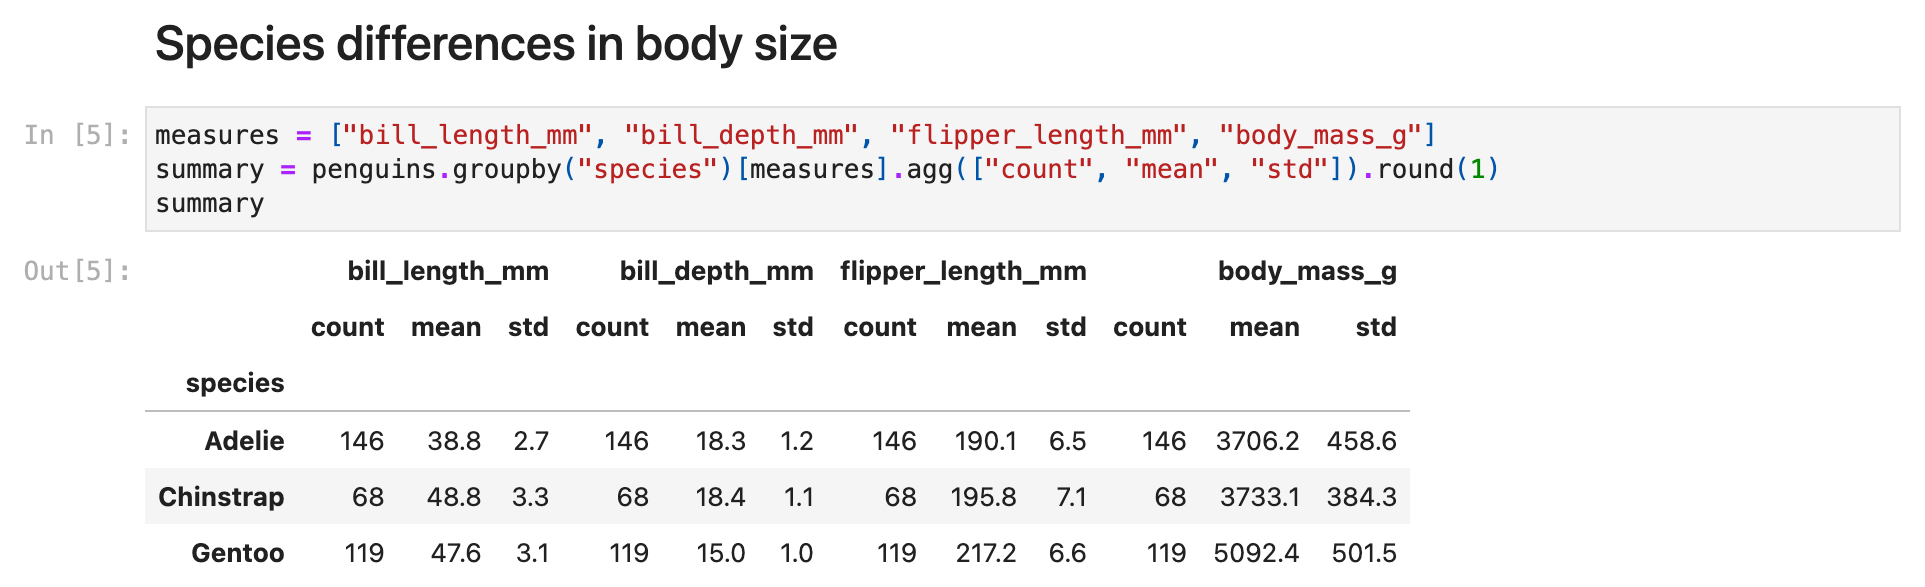
\includegraphics[width=0.78\linewidth]{figures/penguin_notebook_excerpt.png}}\\[0.7em]
    \begin{tikzpicture}[font=\small\sffamily]
      \node[nd box, text width=3.9cm, minimum height=1.4cm, inner sep=5pt] at (-4.4,0) {\textbf{Text cells}\\explain the analysis};
      \node[nd box, text width=3.9cm, minimum height=1.4cm, inner sep=5pt] at (0,0) {\textbf{Code cells}\\numbered, like \texttt{In [5]}};
      \node[nd highlight, text width=3.9cm, minimum height=1.4cm, inner sep=5pt] at (4.4,0) {\textbf{Saved outputs}\\like \texttt{Out [5]}: no need to run};
    \end{tikzpicture}
  \end{center}
  \vspace{1.5cm plus 1fill}
\end{frame}

\begin{frame}{The notebook's analysis, section by section}
  \vfill
  \begin{columns}[c]
    \begin{column}{0.58\textwidth}
      \begin{enumerate}\large\setlength\itemsep{0.5em}
        \item Load and clean
        \item Species differences in body size
        \item Flipper length: Adelie vs Chinstrap
        \item Body mass and sex in Adelie penguins
        \item Differences among islands
        \item Bill length and bill depth
        \item Figure 1
      \end{enumerate}
    \end{column}
    \begin{column}{0.38\textwidth}
      \slidepoint{Summary tables, \textbf{statistical tests}, and two figures.}
    \end{column}
  \end{columns}
  \vspace{1.5cm plus 1fill}
\end{frame}

\begin{frame}[fragile]{The write-up: the claims you will check}
  \vfill
  \begin{columns}[c]
    \begin{column}{0.62\textwidth}
      \begin{lstlisting}[basicstyle=\ttfamily\footnotesize, breaklines=false]
# Body size in three Palmer Archipelago
  penguin species
## 1. Data and methods
## 2. Species differ in body mass
## 3. Flipper length differs between
     Adelie and Chinstrap penguins
## 4. Sex differences in Adelie body mass
## 5. Island effects
## 6. Bill shape
## 7. Figure
## 8. Conclusions
## References
      \end{lstlisting}
      {\small \texttt{writeup.md}: draft results for a group meeting}
    \end{column}
    \begin{column}{0.34\textwidth}
      \textbf{It makes claims:}
      \begin{itemize}\large\setlength\itemsep{0.5em}
        \item numbers
        \item comparisons
        \item interpretations
        \item conclusions
      \end{itemize}
    \end{column}
  \end{columns}
  \vspace{1.5cm plus 1fill}
\end{frame}

\begin{frame}{The figures saved by the notebook}
  \vfill
  \begin{center}
    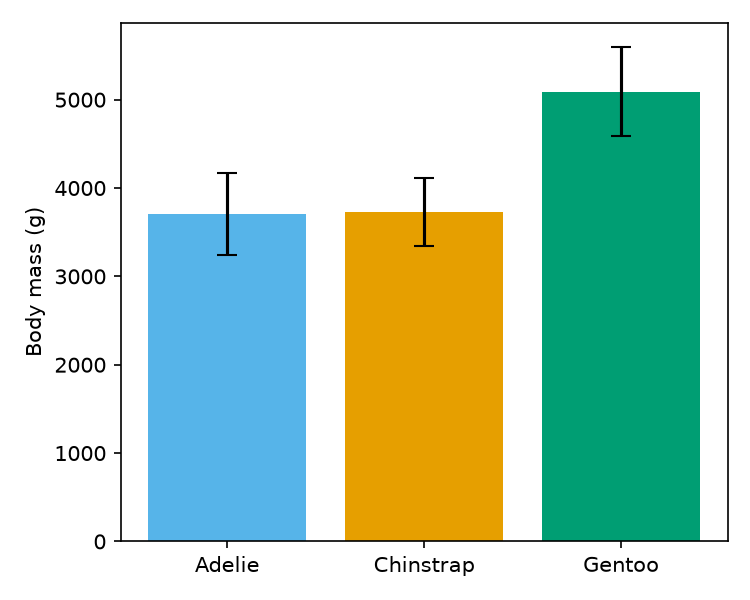
\includegraphics[height=4.9cm]{figures/penguin_body_mass_by_species.png}\hspace{0.8cm}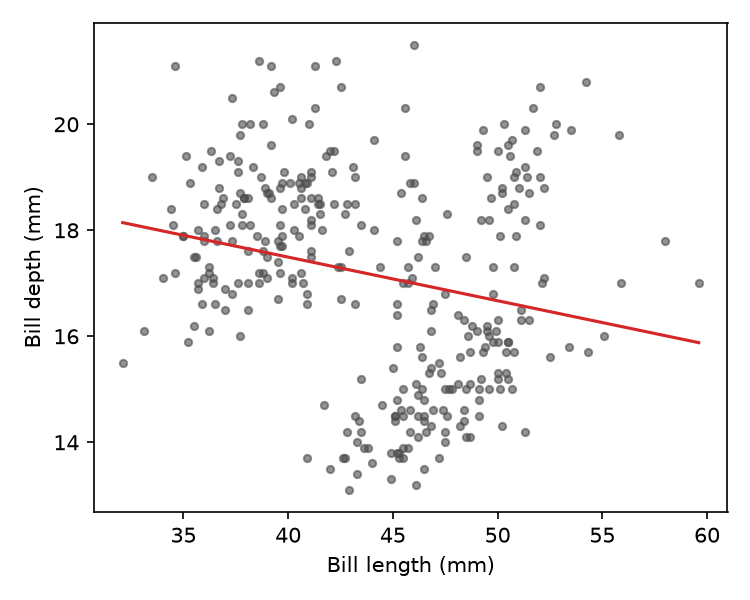
\includegraphics[height=4.9cm]{figures/penguin_bill_length_vs_depth.png}\\[0.5em]
    {\small \texttt{figures/}: two PNG files, one used in the write-up}
  \end{center}
  \vspace{1.5cm plus 1fill}
\end{frame}

\begin{frame}{Activity 2: check a teammate's analysis with an LLM}
  \vfill
  \begin{columns}[c]
    \begin{column}{0.50\textwidth}
      \resizebox{\linewidth}{!}{\begin{tikzpicture}[font=\small\sffamily, >=Stealth]
        \node[nd box, minimum width=4.2cm, minimum height=1.2cm] (a) at (0,1.7) {\textbf{Notebook}\\{\footnotesize with saved outputs}};
        \node[nd box, minimum width=4.2cm, minimum height=1.2cm] (b) at (0,0) {\textbf{Write-up}\\{\footnotesize the claims}};
        \node[nd box, minimum width=4.2cm, minimum height=1.2cm] (c) at (0,-1.7) {\textbf{Reference texts}\\{\footnotesize open statistics sources}};
        \node[nd highlight, minimum width=3.4cm, minimum height=2.4cm] (d) at (6.4,0) {\textbf{An audit}\\{\footnotesize that you}\\{\footnotesize have checked}};
        \draw[->, very thick, NDBlue] (a.east) -- (d.north west);
        \draw[->, very thick, NDBlue] (b.east) -- (d.west);
        \draw[->, very thick, NDBlue] (c.east) -- (d.south west);
      \end{tikzpicture}}
    \end{column}
    \begin{column}{0.46\textwidth}
      \slidepoint{A member of your team gives you \textbf{this notebook} with a statistical analysis.}\\[0.9em]
      {\small How can you use an LLM to \textbf{augment your critical thinking} and check the analysis?}\\[0.9em]
      {\small It contains deliberate problems, some easy and some subtle. We will not say how many.}\\[0.7em]
      {\small Pick up the \textbf{Part 2 handout} and turn to the activity on the back.}
    \end{column}
  \end{columns}
  \vfill
  \ndlogonote{\scriptsize Hands-on: 45 minutes; regroup: 15 minutes}
\end{frame}

\begin{frame}{The setup: the data, the questions, and what to check against}
  \vfill
  \begin{center}
    \begin{tikzpicture}[font=\small\sffamily]
      \node[nd box, text width=0.27\textwidth, minimum height=4.3cm, align=left, inner sep=8pt, anchor=north] at (-0.325\textwidth,0)
        {\textbf{\normalsize The data}\\[0.4em]
         Palmer Penguins\\
         344 penguins, 3 species, 3 islands, 2007--2009\\[0.4em]
         {\footnotesize Bill length and depth, flipper length, body mass, sex\\[0.2em] Public, CC0}};
      \node[nd box, text width=0.27\textwidth, minimum height=4.3cm, align=left, inner sep=8pt, anchor=north] at (0,0)
        {\textbf{\normalsize The questions}\\[0.4em]
         How do the species differ in size?\\[0.3em]
         Do males and females differ?\\[0.3em]
         Do the islands matter?\\[0.3em]
         How are bill length and depth related?};
      \node[nd highlight, text width=0.27\textwidth, minimum height=4.3cm, align=left, inner sep=8pt, anchor=north] at (0.325\textwidth,0)
        {\textbf{\normalsize To check against}\\[0.4em]
         Three open references:\\
         {\footnotesize a statistics textbook, the NIST e-Handbook, the ASA statement on p-values}\\[0.4em]
         The raw data file and its documentation};
    \end{tikzpicture}
  \end{center}
  \vspace{0.6em}
  \begin{center}
    \slidepoint{Decide which claims you would let \textbf{stand}.}
  \end{center}
  \vspace{1.6cm plus 1fill}
\end{frame}

\begin{frame}[fragile]{Get the materials and open the folder in Claude}
  \vfill
  \begin{columns}[c]
    \begin{column}{0.48\textwidth}
      \begin{enumerate}\small\setlength\itemsep{0.6em}
        \item \href{https://github.com/dowlinglab/claude-for-researchers/releases/latest}{\textbf{Download the ZIP}} (address below) and unzip it.
        \item Open the \texttt{audit-project} folder itself in Claude. In a chat app, attach \texttt{writeup.md}, the notebook, and \texttt{data/README.md}.
        \item Paste the \textbf{starter prompt} on the next slide. It includes the reference links.
        \item \textbf{Optional:} save a reference copy in \texttt{references/pdfs/}. If Claude cannot find it, tell it the file name.
      \end{enumerate}
    \end{column}
    \begin{column}{0.50\textwidth}
      \begin{lstlisting}[basicstyle=\ttfamily\scriptsize]
audit-project/
  writeup.md         the claims
  notebooks/         the analysis
  data/              data and README
  figures/           two figures
  references/pdfs/   optional copies
  environment.yml    optional
      \end{lstlisting}
    \end{column}
  \end{columns}
  \vspace{0.4em}
  \begin{center}
    {\small\href{https://github.com/dowlinglab/claude-for-researchers/releases/latest}{\texttt{github.com/dowlinglab/claude-for-researchers/releases/latest}}, under \textbf{Assets}}
  \end{center}
  \vspace{1.6cm plus 1fill}
\end{frame}

\begin{frame}{Start with a prompt that reads before it judges}
  \vfill
  \begin{center}
    \begin{tikzpicture}
      \node[nd box, text width=0.92\linewidth, inner sep=8pt, align=left, font=\small] {\hyphenpenalty=10000\relax
        A teammate sent me this notebook and write-up. I want to audit the analysis, not fix it. Read the write-up, the notebook, and the data documentation, and change nothing. List each substantive claim and where it appears. Then give each claim a status (supported, questionable, incorrect, or insufficient evidence). Say whether you checked it against the notebook's output, the raw data, or a reference, cite the section you relied on, and tell me what you could not open or check. References: the files in \texttt{references/pdfs/}, or these links: \texttt{openintro-ims.netlify.app}, \texttt{itl.nist.gov/div898/handbook}, \texttt{amstat.org/asa/files/pdfs/p-valuestatement.pdf}.};
    \end{tikzpicture}
  \end{center}
  \vspace{0.5em}
  \begin{center}
    \slidepoint{Ask for the \textbf{evidence} and its \textbf{location}, not just a verdict.}\\[0.4em]
    {\small One message covers Steps 1 to 3. Edit it freely, and ask what any unfamiliar term means.}
  \end{center}
  \vspace{1.6cm plus 1fill}
\end{frame}

\begin{frame}{Ask, inspect, verify, iterate}
  \vfill
  \begin{center}
    \resizebox{0.94\linewidth}{!}{\begin{tikzpicture}[font=\normalsize\sffamily, >=Stealth]
      \node[nd box, minimum width=3.4cm, minimum height=2.3cm] (n1) at (0,0) {\textbf{Ask}\\[2pt]{\footnotesize list the claims,}\\{\footnotesize check them against}\\{\footnotesize the references}};
      \node[nd box, minimum width=3.4cm, minimum height=2.3cm] (n2) at (4.4,0) {\textbf{Inspect}\\[2pt]{\footnotesize read every finding}\\{\footnotesize and where it points}};
      \node[nd highlight, minimum width=3.4cm, minimum height=2.3cm] (n3) at (8.8,0) {\textbf{Verify}\\[2pt]{\footnotesize open the reference,}\\{\footnotesize recompute the number}};
      \node[nd box, minimum width=3.4cm, minimum height=2.3cm] (n4) at (13.2,0) {\textbf{Iterate}\\[2pt]{\footnotesize sharpen the prompt,}\\{\footnotesize add context, repeat}};
      \foreach \a/\b in {1/2, 2/3, 3/4} { \draw[->, very thick, NDBlue] (n\a) -- (n\b); }
    \end{tikzpicture}}
  \end{center}
  \vspace{1.1em}
  \begin{center}
    \bad{Prompt $\rightarrow$ trust $\rightarrow$ done}\\[0.9em]
    {\small Ask for a status on every claim: supported, questionable, incorrect, or insufficient evidence.}
  \end{center}
  \vspace{1.4cm plus 1fill}
\end{frame}
\begin{frame}{Give every claim one of four statuses}
  \vfill
  \renewcommand{\arraystretch}{1.5}
  \begin{center}
    \small
    \begin{tabular}{@{}p{3.2cm}p{9.2cm}@{}}
      \toprule
      \textbf{Status} & \textbf{Use it when}\\
      \midrule
      Supported & The notebook's output, the data, or a cited reference agrees. Ask which.\\
      Questionable & The claim may hold, but the wording or method is doubtful.\\
      Incorrect & The evidence or a cited reference contradicts the claim.\\
      Insufficient evidence & These files cannot show it either way. This is not the same as wrong.\\
      \bottomrule
    \end{tabular}
  \end{center}
  \vspace{0.8em}
  \begin{center}
    \slidepoint{\textbf{Insufficient evidence} is a result, not a failure.}
  \end{center}
  \vspace{1.6cm plus 1fill}
\end{frame}

\begin{frame}[fragile]{Optional Step 0: make agent changes easy to review}
  \vfill
  \begin{columns}[c]
    \begin{column}{0.44\textwidth}
      {\small\textbf{Optional, if you are comfortable with Git and Python.}\\
      If not, skip it. You are not behind.}\\[0.8em]
      \begin{enumerate}\small\setlength\itemsep{0.35em}
        \item Commit a clean \textbf{baseline} before anything changes.
        \item Move the analysis code into readable \textbf{Python files}.
        \item Commit the refactor \textbf{separately}.
        \item Then start the audit.
      \end{enumerate}
    \end{column}
    \begin{column}{0.54\textwidth}
      {\footnotesize\textbf{Notebook:} change one number, rerun}
      \begin{lstlisting}[basicstyle=\ttfamily\scriptsize, aboveskip=0.1em, belowskip=0.2em]
- "image/png": "iVBOR..." [34,731 chars]
+ "image/png": "iVBOR..." [35,271 chars]
- "ax.scatter(...\"depth\"], s=12,...
+ "ax.scatter(...\"depth\"], s=16,...
      \end{lstlisting}
      {\footnotesize\textbf{Python file:} the same change}
      \begin{lstlisting}[basicstyle=\ttfamily\scriptsize, aboveskip=0.1em, belowskip=0.2em]
-  ax.scatter(x, y, s=12, alpha=0.6)
+  ax.scatter(x, y, s=16, alpha=0.6)
      \end{lstlisting}
    \end{column}
  \end{columns}
  \vspace{0.3em}
  \begin{center}\small
    The right format depends on the task. For heavy agent editing, plain text is easier to audit.
  \end{center}
  \vspace{0.6cm plus 1fill}
\end{frame}
\begin{frame}{Then judge the audit itself}
  \vfill
  \begin{columns}[c]
    \begin{column}{0.50\textwidth}
      \slidepoint{Keep a \textbf{log}: finding, evidence, how you checked it.}\\[0.9em]
      {\small Verify at least \textbf{three} findings yourself: a number, a citation, and a claim marked \emph{Supported}.}\\[0.6em]
      {\small Note which model and setup you used.}\\[0.6em]
      {\small Save your log at minute 40.}
    \end{column}
    \begin{column}{0.46\textwidth}
      \begin{itemize}\small\setlength\itemsep{0.55em}
        \item What did it find, and what did it miss?
        \item Did it invent anything?
        \item Were its citations accurate?
        \item What improved it?
      \end{itemize}
    \end{column}
  \end{columns}
  \vspace{1.4cm plus 1fill}
\end{frame}
